%General
\documentclass{article}
\usepackage[utf8]{inputenc}
\usepackage{fullpage}

%Symbols
\usepackage{commath}
\usepackage{amsmath}
\usepackage{amssymb}
\usepackage{tikz}
\usetikzlibrary{arrows,automata}

%Numbering
\usepackage{chngcntr}
\counterwithin{figure}{section}
\usepackage{enumerate}

%Formatting
\usepackage{bussproofs}
\usepackage{hyperref}
\usepackage{amsthm}
\usepackage{alltt}
\newtheorem{theorem}{Theorem}[section]
\newtheorem{definition}[theorem]{Definition}
\newtheorem{example}[theorem]{Example}
\hypersetup{colorlinks=true}
\hypersetup{colorlinks=true}
\usepackage{graphicx}
\graphicspath{ {img/} }
\usepackage{caption}

\title{Week 4: Regular Languages}
\date{\today}
\author{Rikard Hjort}

\begin{document}
\maketitle

\section{}

For clarity moving forward, I will set up the following names:

\begin{align*}
    R &= (a+b)^* \\
    S &= (b^*a^*)^* \\
    \Sigma &= \set{a,b}
\end{align*}

There are several ways that we could prove that $L(R)=L(S)$. We could do this for example by induction on the length of a string or by structural induction on $\Sigma^*$ to prove that $L(R) = \Sigma^*$ and $L(S) = \Sigma^*$. However, for this excericise I will prove their equivalence by constructing FA's which I will show are equivalent.

By using the standard inductive way of creating an $\epsilon$-NFA $E_1$ from a RE, we create the automaton in figure \ref{fig:aplusb} from $R$.

\begin{figure}[htpb]
    \centering
    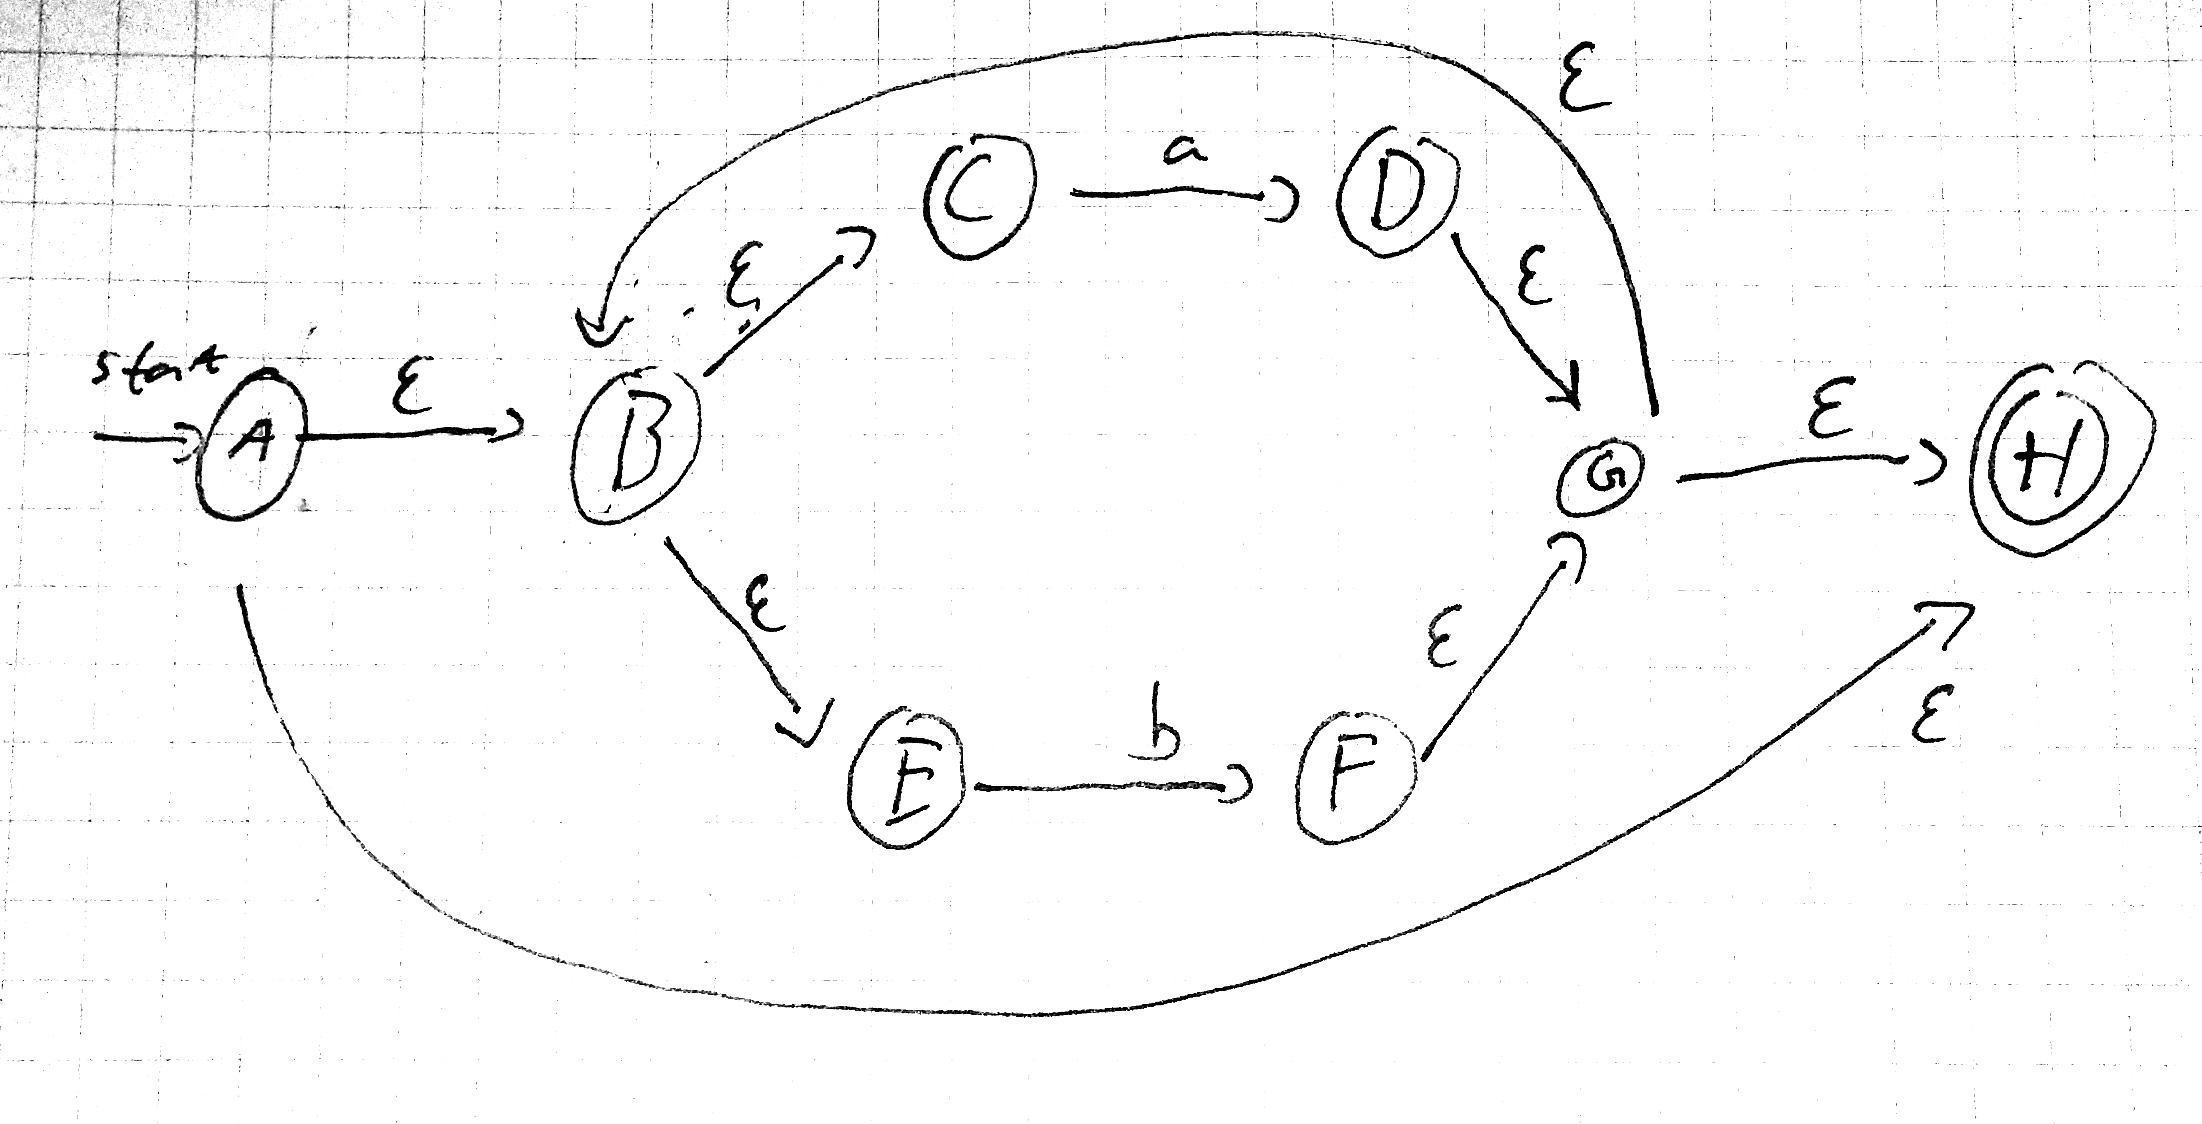
\includegraphics[width=0.8\linewidth]{aplusb}
    \caption{The $\epsilon$-NFA $E_1$ generated by the standard method from the expression $(a+b)^*$.}
    \label{fig:aplusb}
\end{figure}

In this automaton, states $B$ through $G$ represent the expression $a+b$, if you exclude the the arc from $G$ to $B$. That arc, together with states $A$ and $H$ and all transitions from and to them, represent the entire expression.

Through the standard construction of DFA from $\epsilon$-NFA described in section 2.5.5 of the course book, we turn $E_1$ into a DFA $D_1$. First we $\epsilon$-close the start state, obtaining a new state in $D_1$: $\set{A,B,C,E,H}$. From this, we try all symbols in $\Sigma$ and see that on the input $a$ we transition to the state $\set{B,C,D,E,G,H}$. If we read $b$ we transition to $\set{B,C,D,F,G,H}$. Taking into account the transitions from these two new states, we arrive at the automaton in figure \ref{fig:aplusbmin}.

\begin{figure}[htpb]
    \centering
    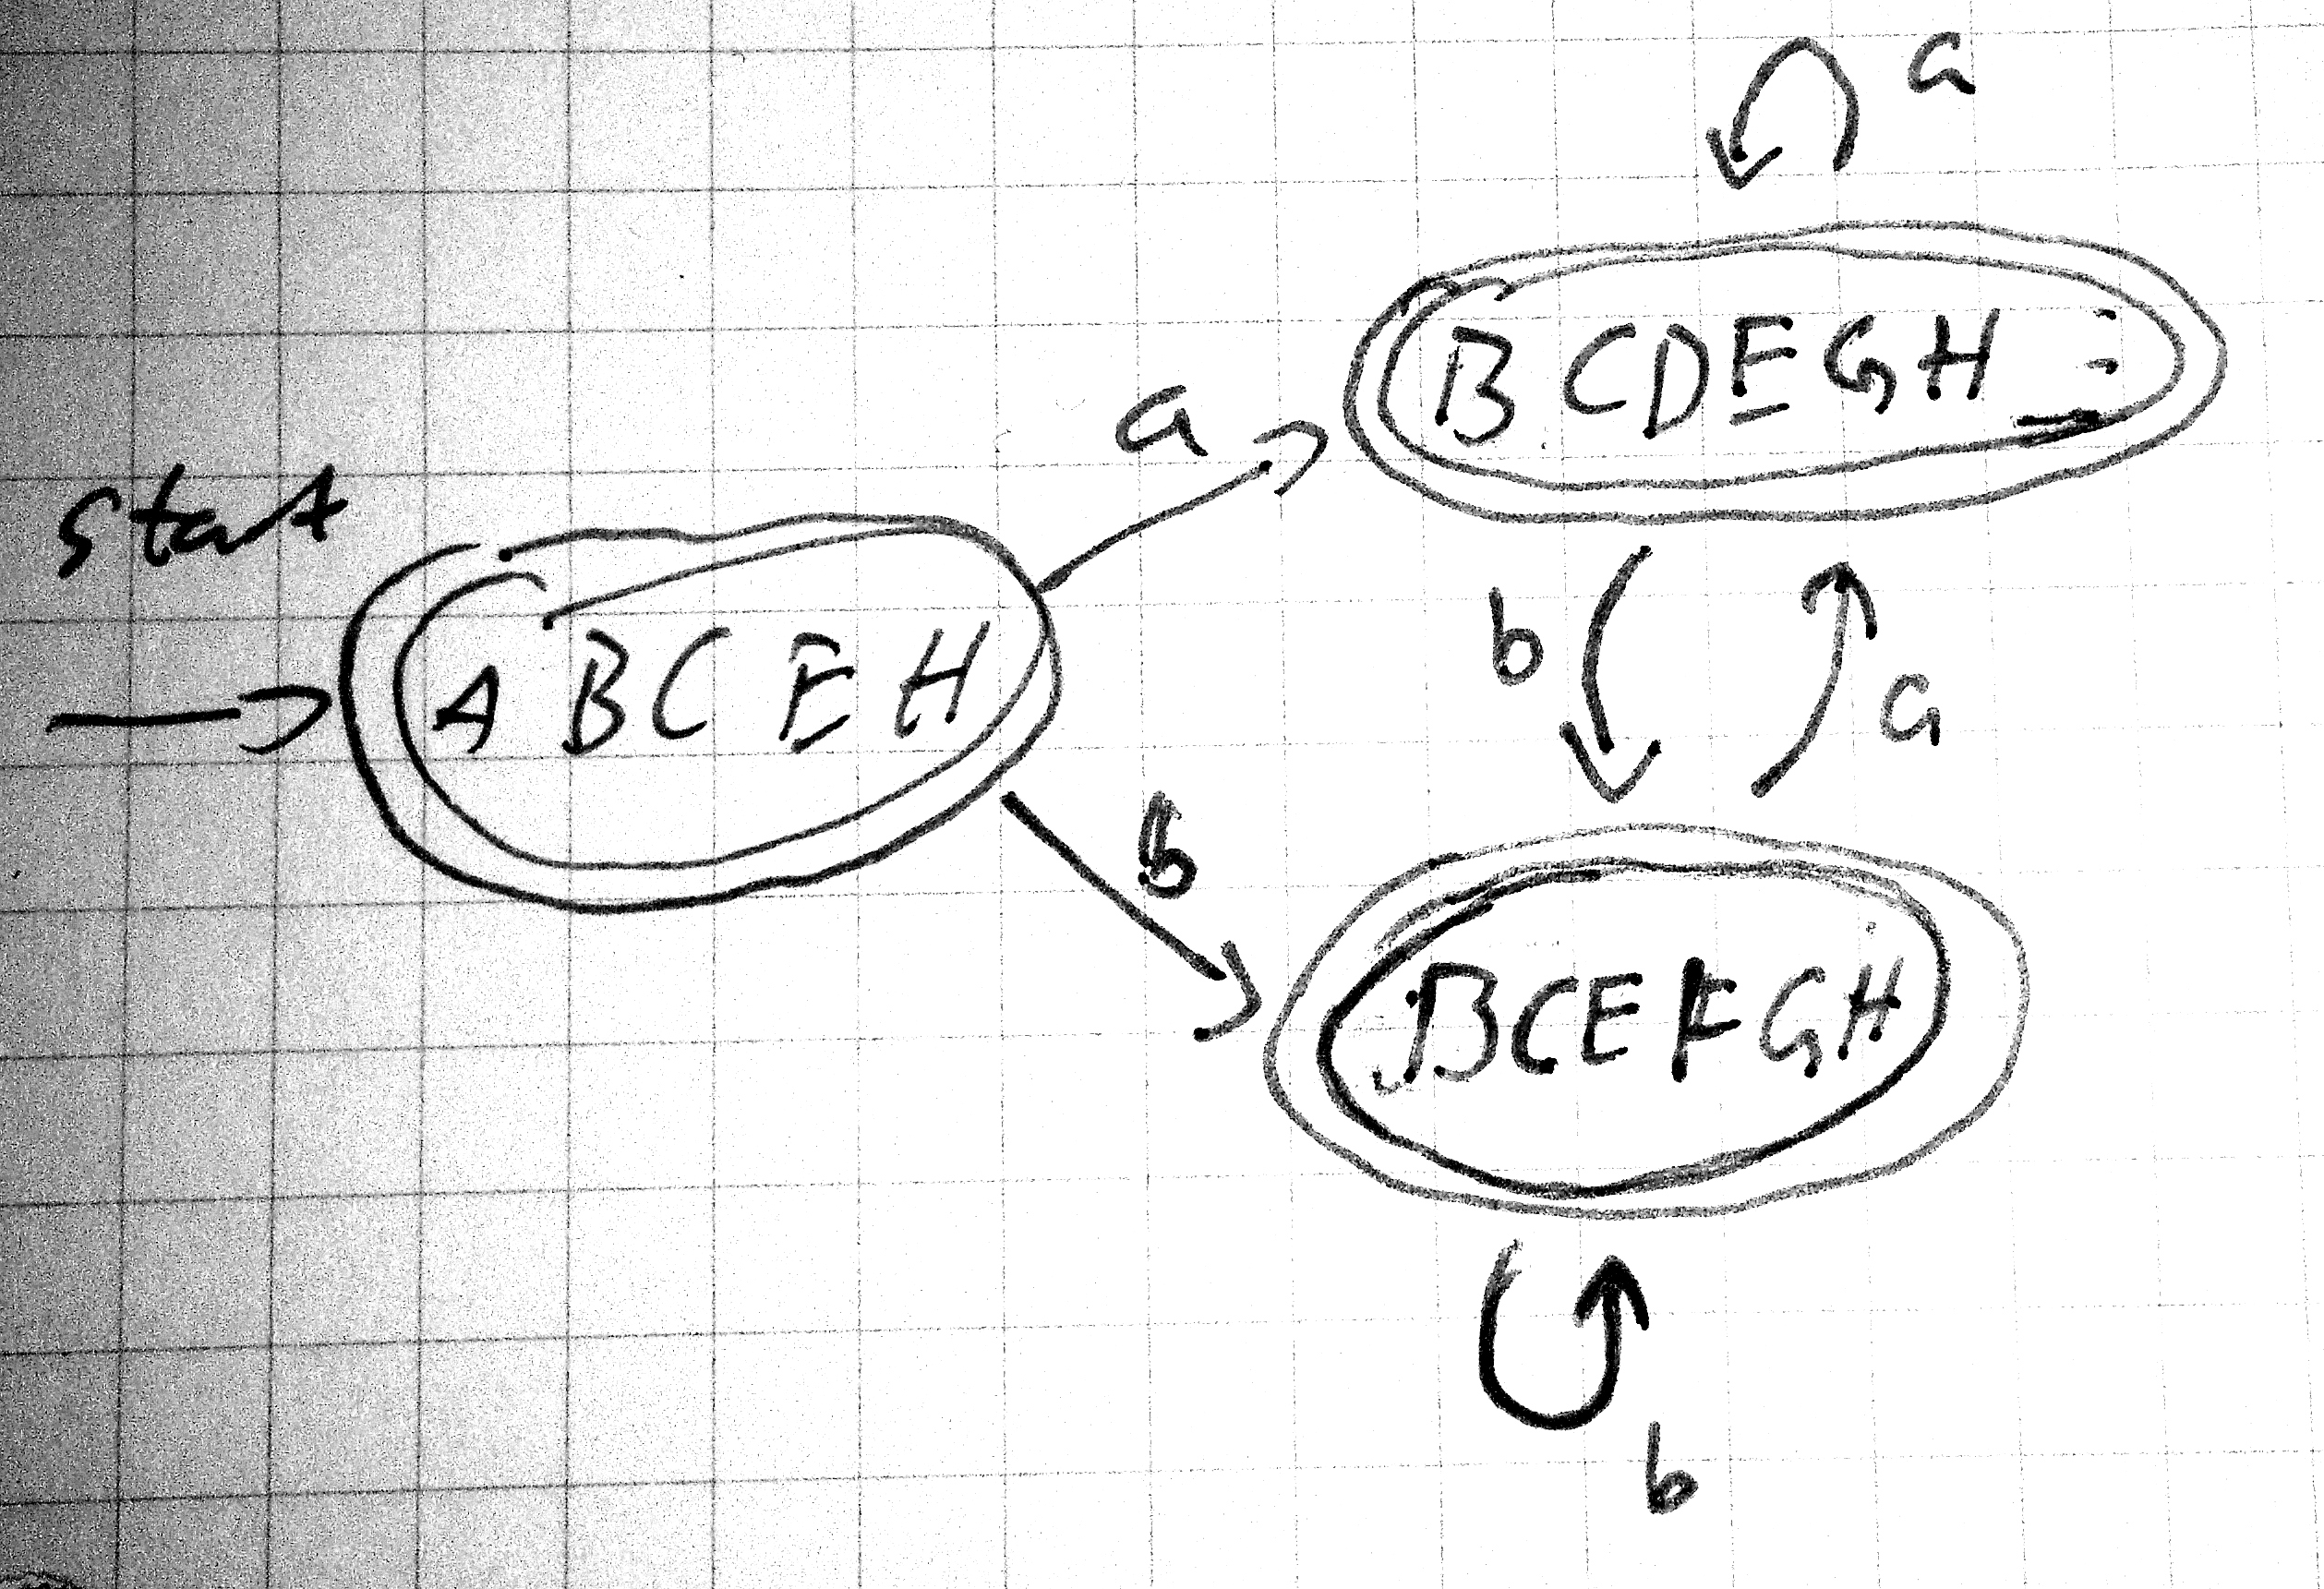
\includegraphics[width=0.6\linewidth]{aplusbmin}
    \caption{The DFA $D_1$ resulting from elimination of $\epsilon$-transitions of the FA in figure \ref{fig:aplusb}.}
    \label{fig:aplusbmin}
\end{figure}
\bibliography{Bibl}

Since this is a DFA, which always transitions to a new state, and since every reachable state is accepting, we can conclude that this DFA, and therefore $R$, must accept every input string of symbols from the alphabet in question, $\Sigma$. For clarity, we can minimize this DFA. This turns out to be trivial. Since ecery state is accepting, they are pairwise not distinguishable. And since no state is distinguishable from any other even on the first run-through of all the states, all the states are equilvalent. We can reduce $D_1$ to the automaton in figure \ref{fig:minimizedfinal}, by merging the three states to a single one and renaming it $q$.

\begin{figure}[htpb]
    \centering
    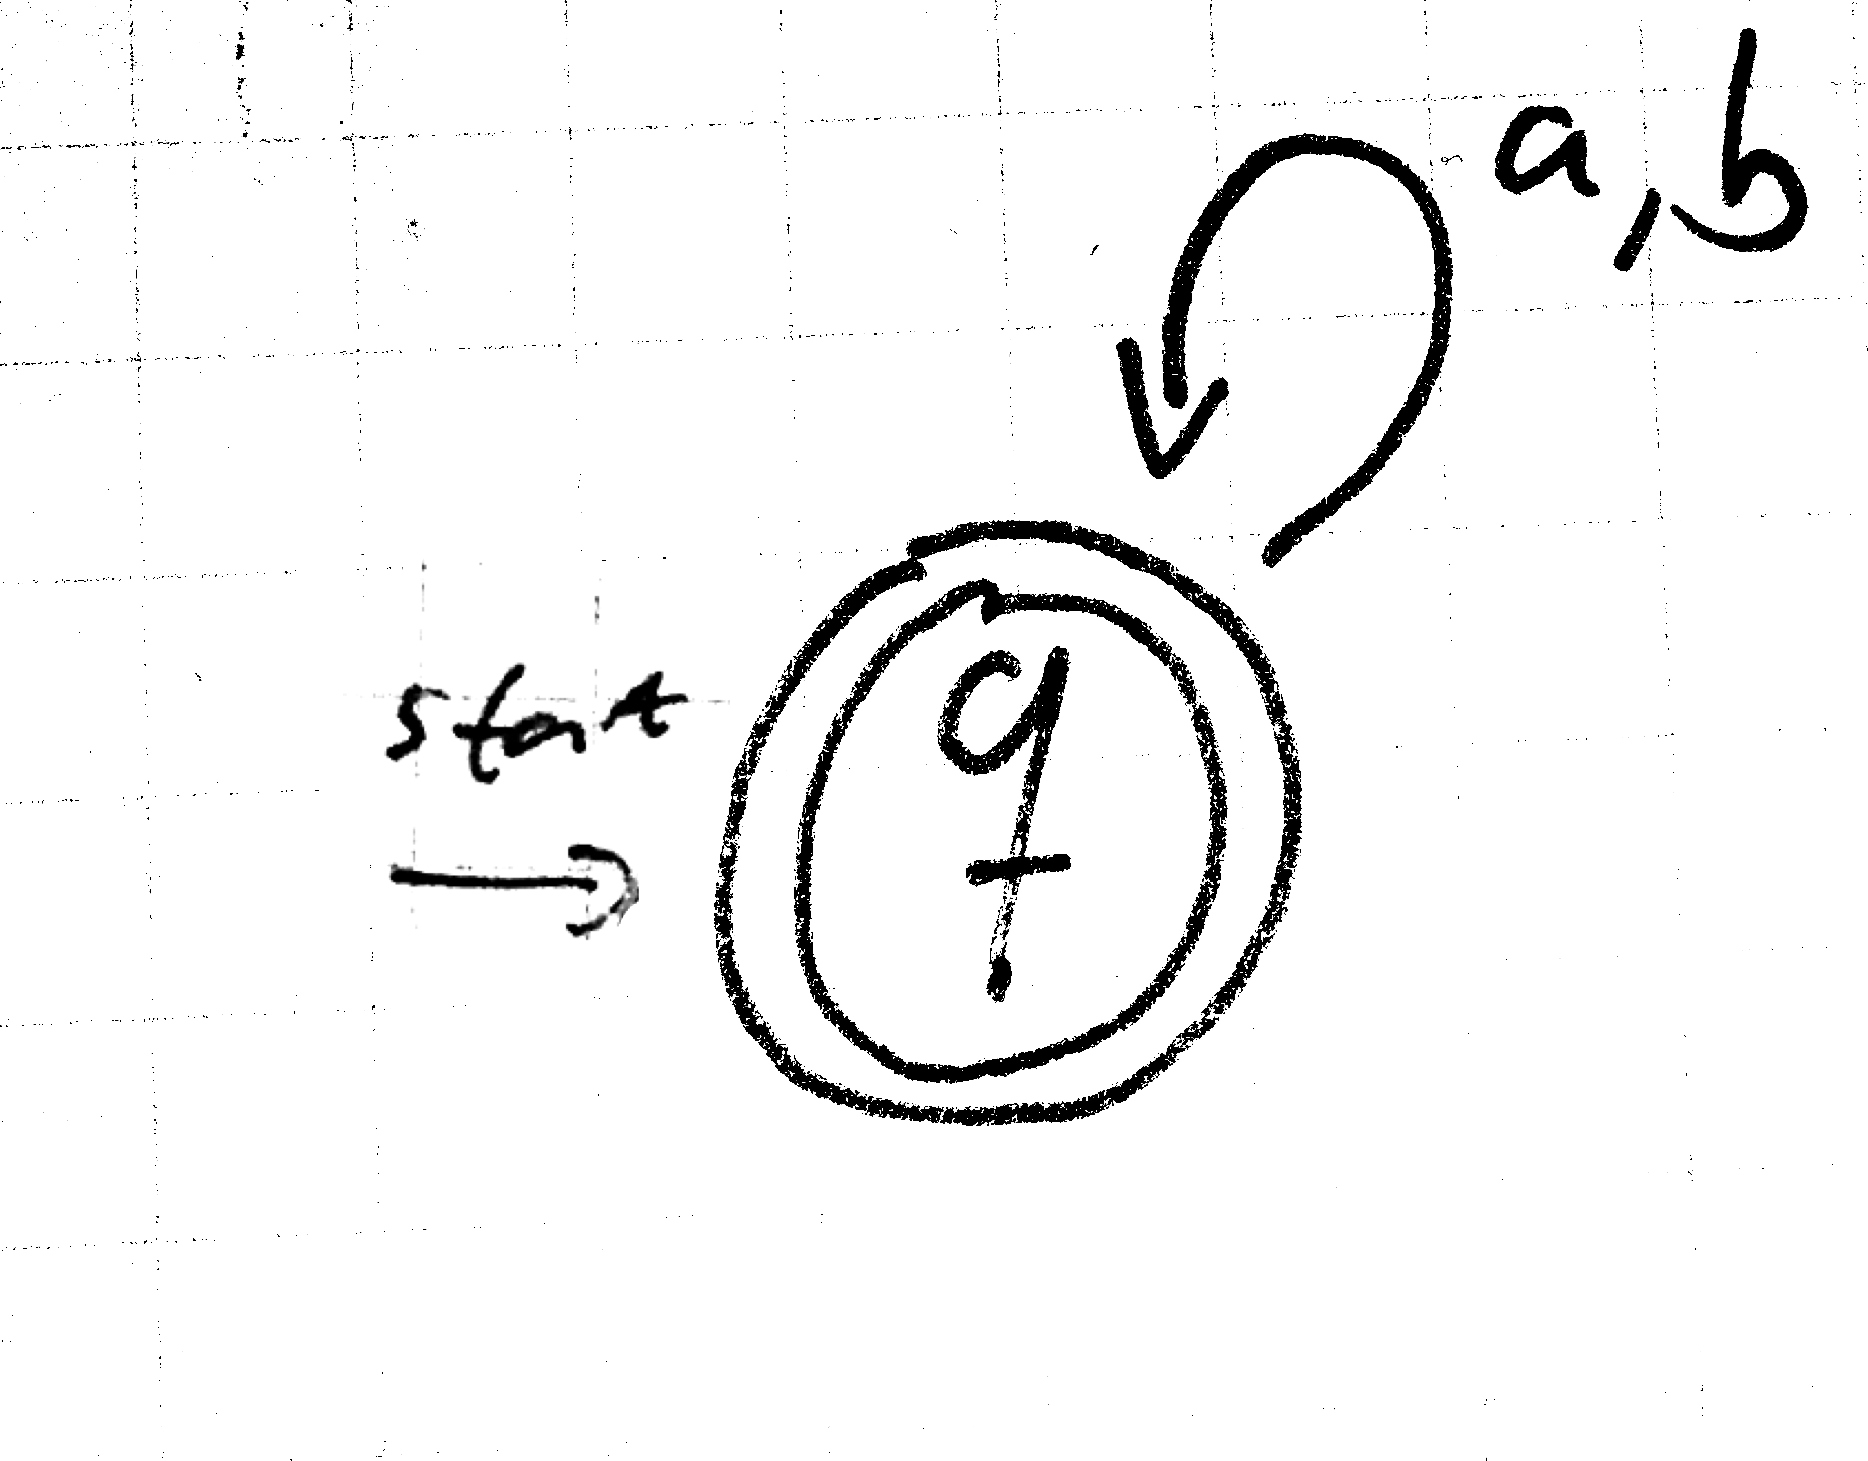
\includegraphics[width=0.3\linewidth]{minimizedfinal}
    \caption{The minimization of $D_1$}
    \label{fig:minimizedfinal}
\end{figure}

We will now repeat the same procedure with $S$. Since we are done with $E_1$, I will reuse the state names from $E_1$ when constructing $E_2$, but these states are not to be confused with each other.

First, we construct the $\epsilon$-NFA $E_2$ in the standard fashion. $E_2$ is made from the closure of the concatenation of the closures of two symbols. $E_2$ is shown in figure \ref{fig:bastar}.

\begin{figure}[htpb]
    \centering
    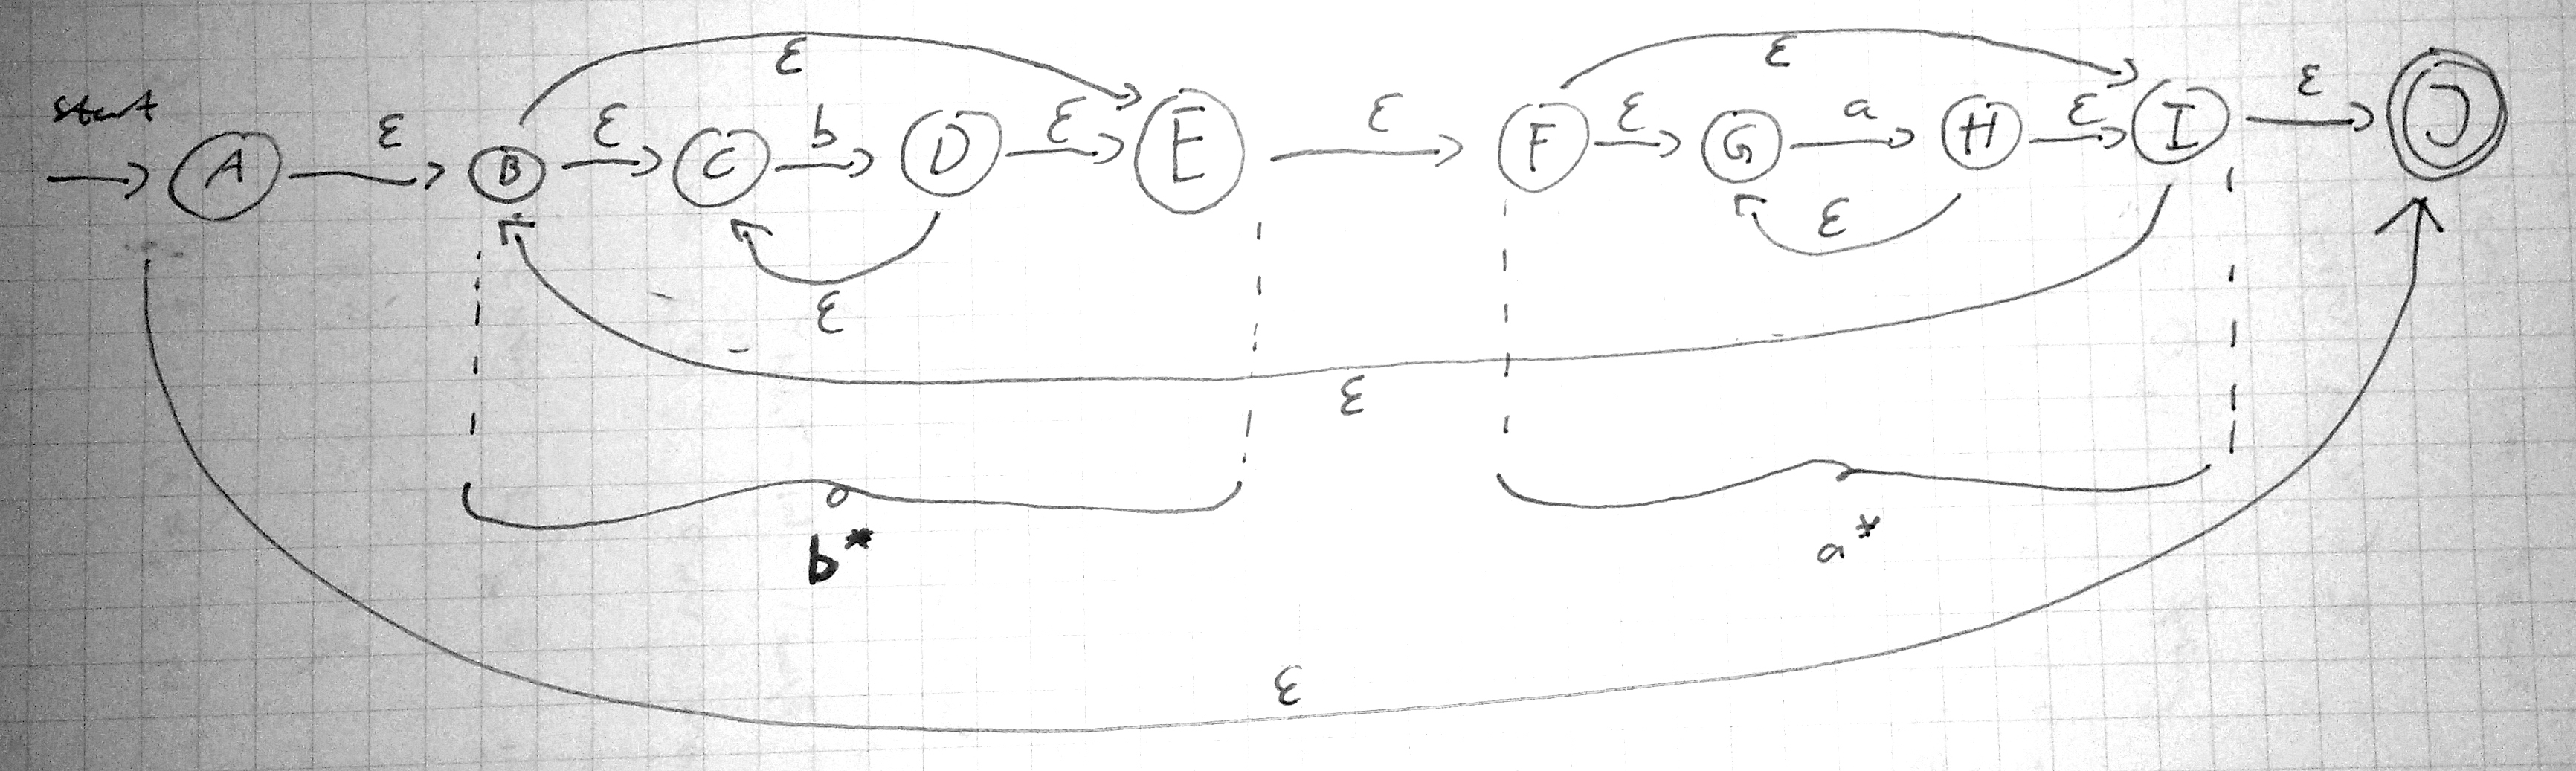
\includegraphics[width=\linewidth]{bastar}
    \caption{The $\epsilon$-NFA constructed from the expression $(b^*a^*)^*$. Brackets denoting the sub-automata for $b^*$ and $a^*$ have been added for clarity.}
    \label{fig:bastar}
\end{figure}
\bibliographystyle{ieeetr}

Eliminating $\epsilon$-transitions we obtain the DFA $D_2$. Its starting state is

$$ECLOSE(A) = \set{A,B,C,E,F,G,I,J}$$

From the starting state we can transition to $\set{B,C,D,E,F,G,I,J}$ on input $a$ or $\set{B,C,E,F,G,H,I,J}$ on input $b$. We then transition back and forth between the two latter states on all inputs.

The resulting DFA is shown in figure \ref{fig:bastarmin}.

\begin{figure}[htpb]
    \centering
    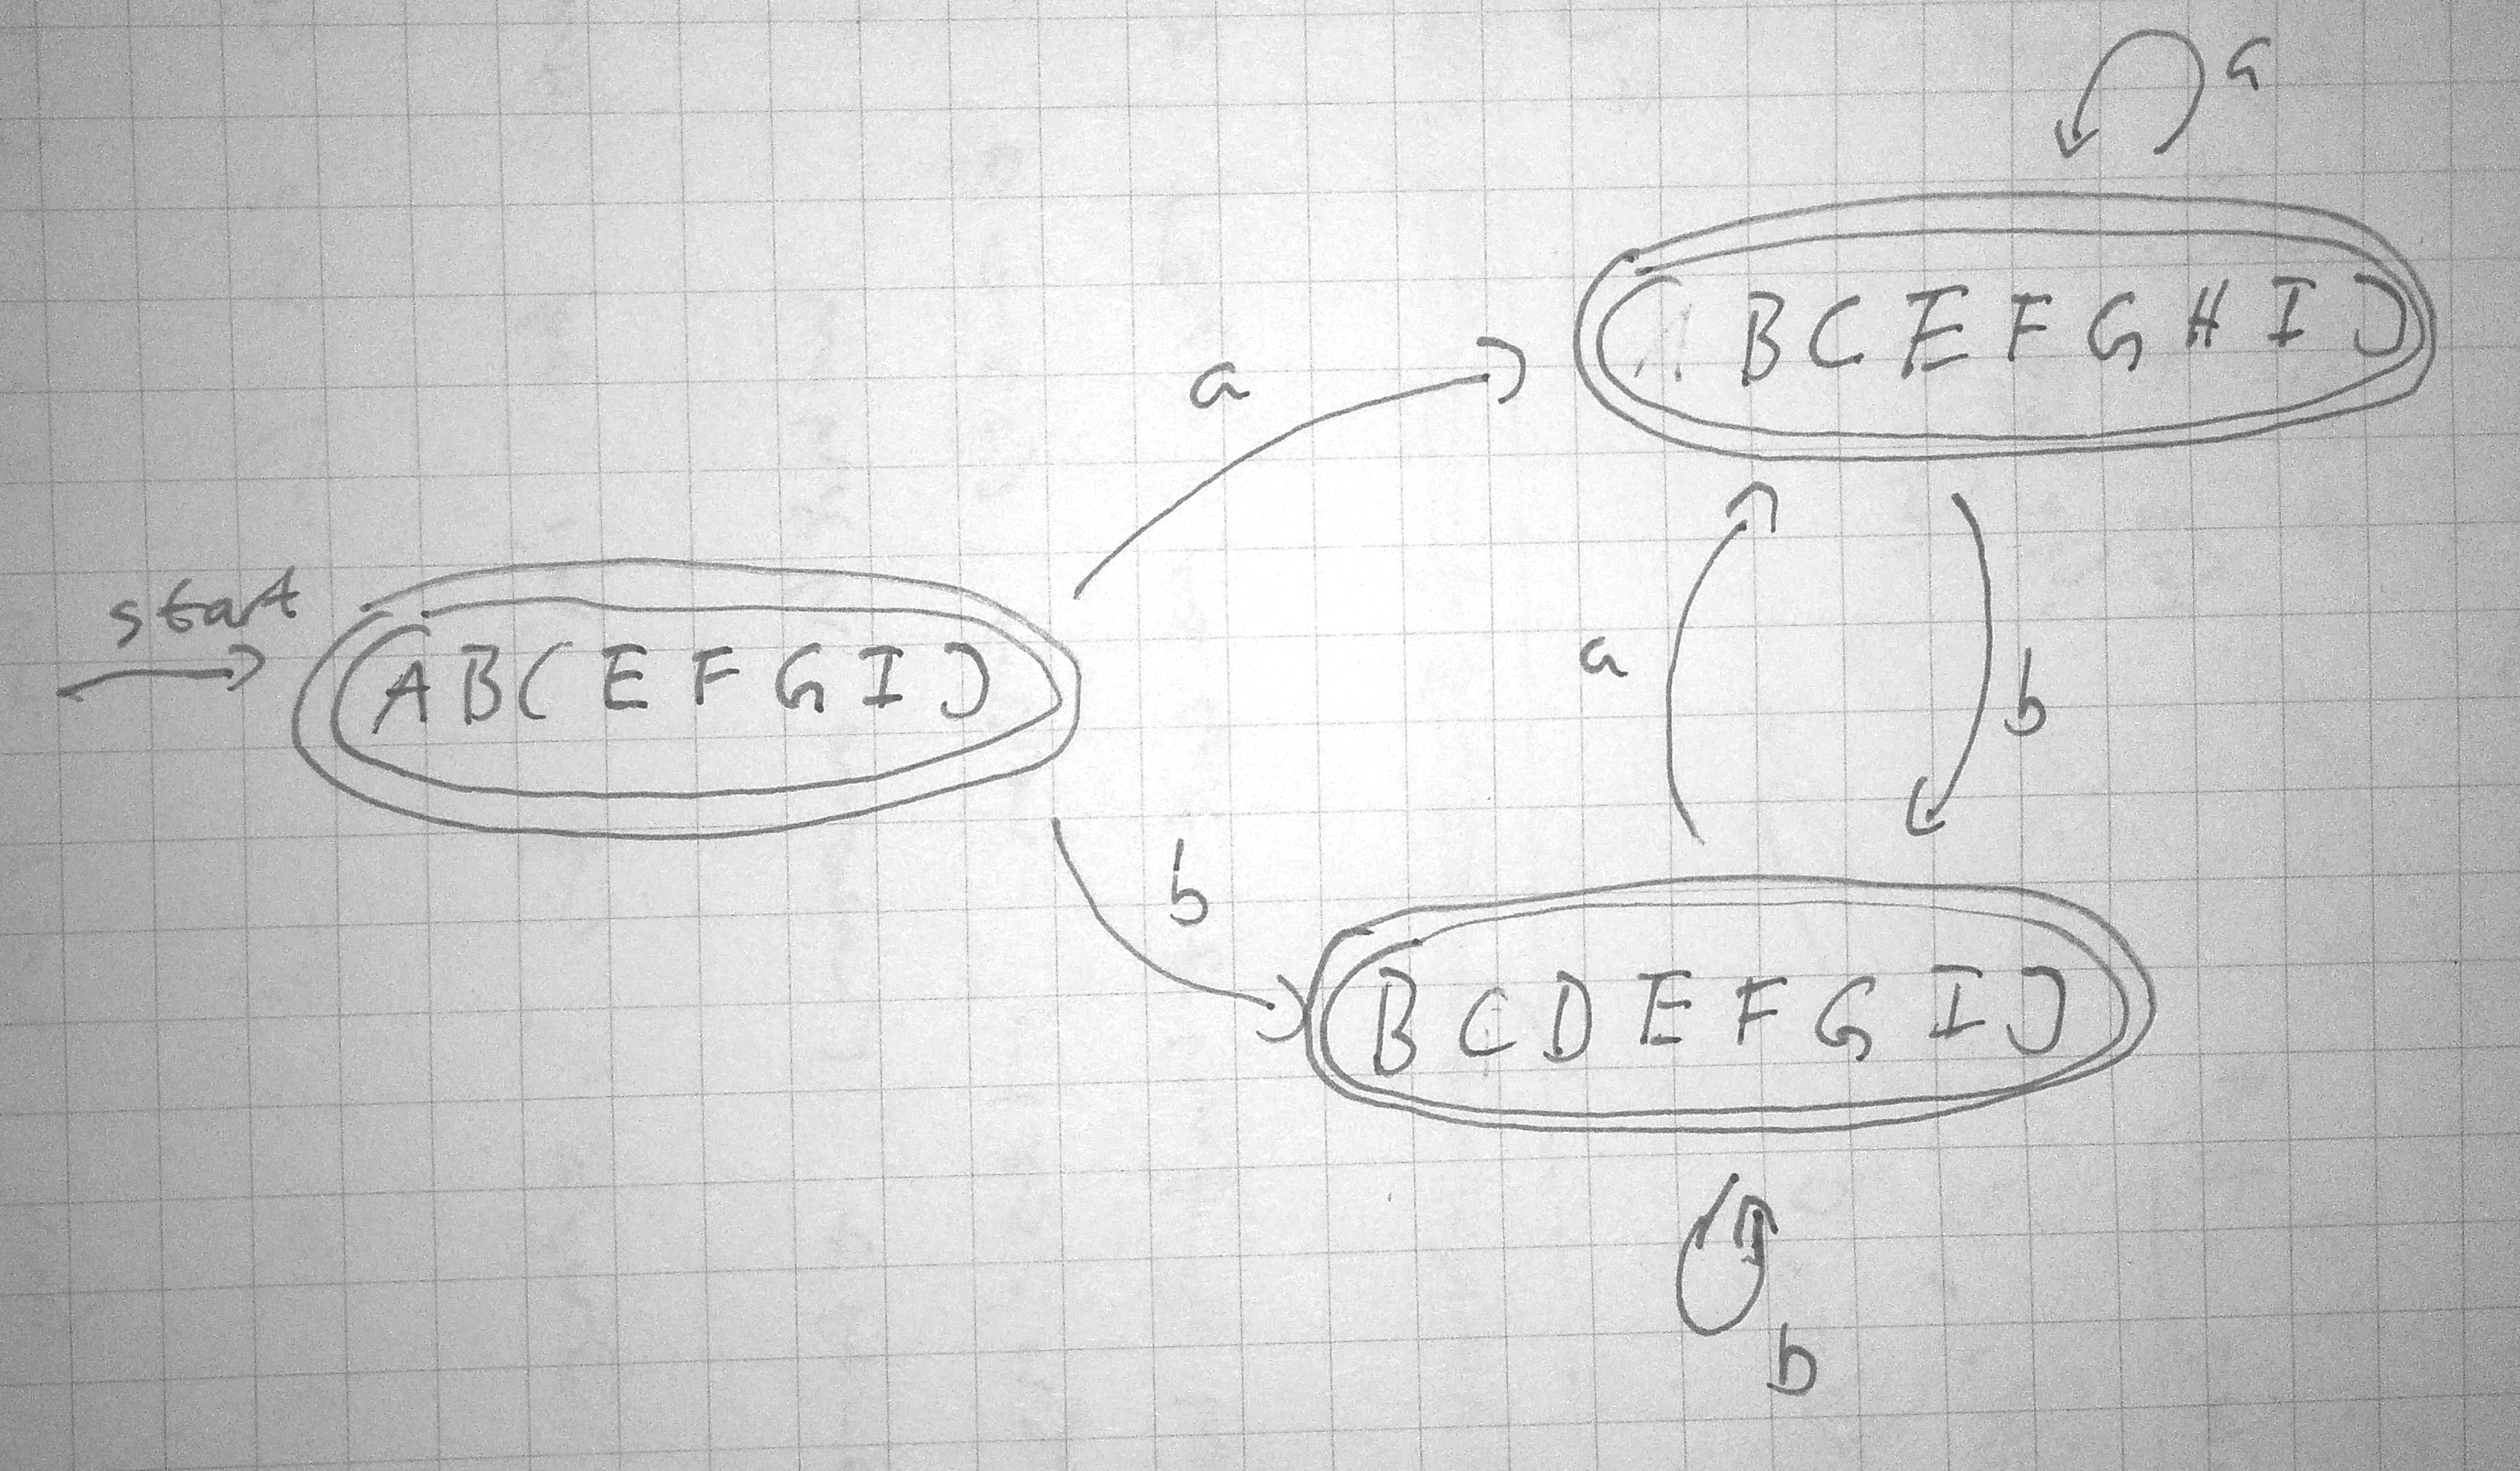
\includegraphics[width=0.8\linewidth]{bastarmin}
    \caption{The DFA $D_2$ which resulting from eliminating $\epsilon$-transitions in the DFA in figure \ref{fig:bastar}.}
    \label{fig:bastarmin}
\end{figure}

Once again we note that every reachable state is accepting, and thus that $S$ accepts all strings made from symobls in $\Sigma$. If we were to minimize this automaton, we would find that every state is pairwise indistinguishable, and that we therefore can replace $D_2$ with the automaton in figure \ref{fig:minimizedfinal}, after renaming the single remaining state to $q$.

We have found that both $R$ and $S$ accept the same language as $D_1$ and $D_2$ respectively, by the theorems of constructing $\epsilon$-NFA from RE and DFA from $\epsilon$-NFA. We have further found $D_1$ and $D_2$ to be equivalent, since through minimization they are turned into the same automaton. Therefore, $R$ and $S$ are equivalent and represent the same language.

\newpage
\section{}

We have shown that the language $L_1 = \set{0^n1^n | n \geq 0}$ is not
regular.\footnote{In short, this can be done through the pumping lemma by
picking the string $0^m1^m$, which is i in $L_2$, for $m$ which is equal to the
constant in the pumping lemma, and showing that pumping any such string would
result in strings $0^i1^j$, where $i \neq j$. However, since this has been done
in the course book, and, I believe, also in lectures, I will not detail the
proof here.} Let $L_2 = \set{0^n1^n | n \geq 1}$.  We also
see that $L_2$ can not be regular: the proof is completely analogous to that for $L_1$.

Now, let

$$L = L_1 - L_2$$

By definition $A - B = A \cap \bar{B}$ for all sets $A$ and $B$. Then $L = L_1
\cap \bar{L_2}$. Then $0^01^0=\epsilon$ is in $L_1$, but not in $L_2$,
and is therefore in $L$. For all other strings in $L_1$,
they are also in $L_2$ and thus not in $\bar{L_2}$, and therefore not in $L$.
We conclude that $L = \set{\epsilon}$. Now $L$ is obviously a regular
language\footnote{As are all finite languages of finite strings.}. For example,
it is accepted by the regular expression $\mathbb{\epsilon}$.

\newpage
\section{}

\begin{enumerate}[(a)]
    \item
        We begin by assuming that $L_1$ is regular. If $L_1$ is regular, then the pumping lemma holds for $L_1$. Let $n$ be the constant of the pumping lemma, for which all string as long or longer than $n$ can be divided and pumped.

        Now let $w = 1^n0^{n+1}$. Since $n = \#_1(w) < \#_0(w) = n+1$, $w$ is in $L_1$. Now we say $w =xyz$ in such a way that the following holds, which the pumping lemma tells us is possible for some values of $x,y$ and $z$:

        \begin{enumerate}[(1)]
            \item $y \neq \epsilon$
            \item $|xy| \leq n$
            \item $\forall i \in \mathbb{N}: xy^iz \in L_1$
        \end{enumerate}

        By condition (2), it must be that $xy$ is a string of only 1's, since $w$ begins with exactly $n$ 1's. This in turn, taken with condition (1), means $y$ is one or more 1's. Now, since $xyz$ is in $L_1$, by (3) so is $xy^2z = xyyz$.

        Howevever, since $y$ consists only of 1's, it must be that $\#_1(xyz) < \#_1(xyyz)$, so $ n < \#_1(xyyz) \Rightarrow n + 1 \leq \#_1(xyyz)$. But since all 0's in $xyyz$ are in $z$, $\#_0(xyyz) = \#_0(xyz) = n + 1$. This means that $\#_1(xyyz) \geq \#_0(xyyz)$, which violates the condition for being in $L_1$, so $xyyz$ is not in $L_1$, even though $xyz$ is. Then the pumping lemma does not hold for $L_1$.

        We know that the statement "if $L_1$ is regular, then the pumping lemma holds for $L_1$" is true. Conversely, this means that "if the pumping lemma doesn't hold for $L_1$, then $L_1$ is not regular". We have proven that the pumping lemma doesn't hold for $L_1$, and therefore $L_1$ is not regular by modus ponens.


    \item
        If $R = 1^* + 1^*01^* + 1^*01^*01^*$, then $L(R) = L_2$. This RE generates all strings with none, exactly one or exactly two 0's in it, which is what the condition for being in $L_2$ is.

        If $S = 0 + 00 + 100 + 010 + 001$, then $L(S) = L_1 \cap L_2$. This intersection is all the strings for which the number of 0's is strictly larger than the number of ones, and for which the number of 0's are less than 3. If there are no 0's, then the number of 0's and 1's are equal, or there are more 1's. It follows that the number of 0's must be one or two. 
        
        In the case where the string is a single 0, there can be no 1, for then they would be equal in number. When there are two 0's, we can have none or one 1's. That is, from the expression $1^*01^*01^*$ we may choose only one of 1 and repeat it only once, or we may choose to pick no 1's at all. The result is $S$.
\end{enumerate}

\newpage
\section{}

The resulting table of the table filling algorithm is in figure \ref{fig:table-filling}.

\begin{figure}[htpb]
    \centering
    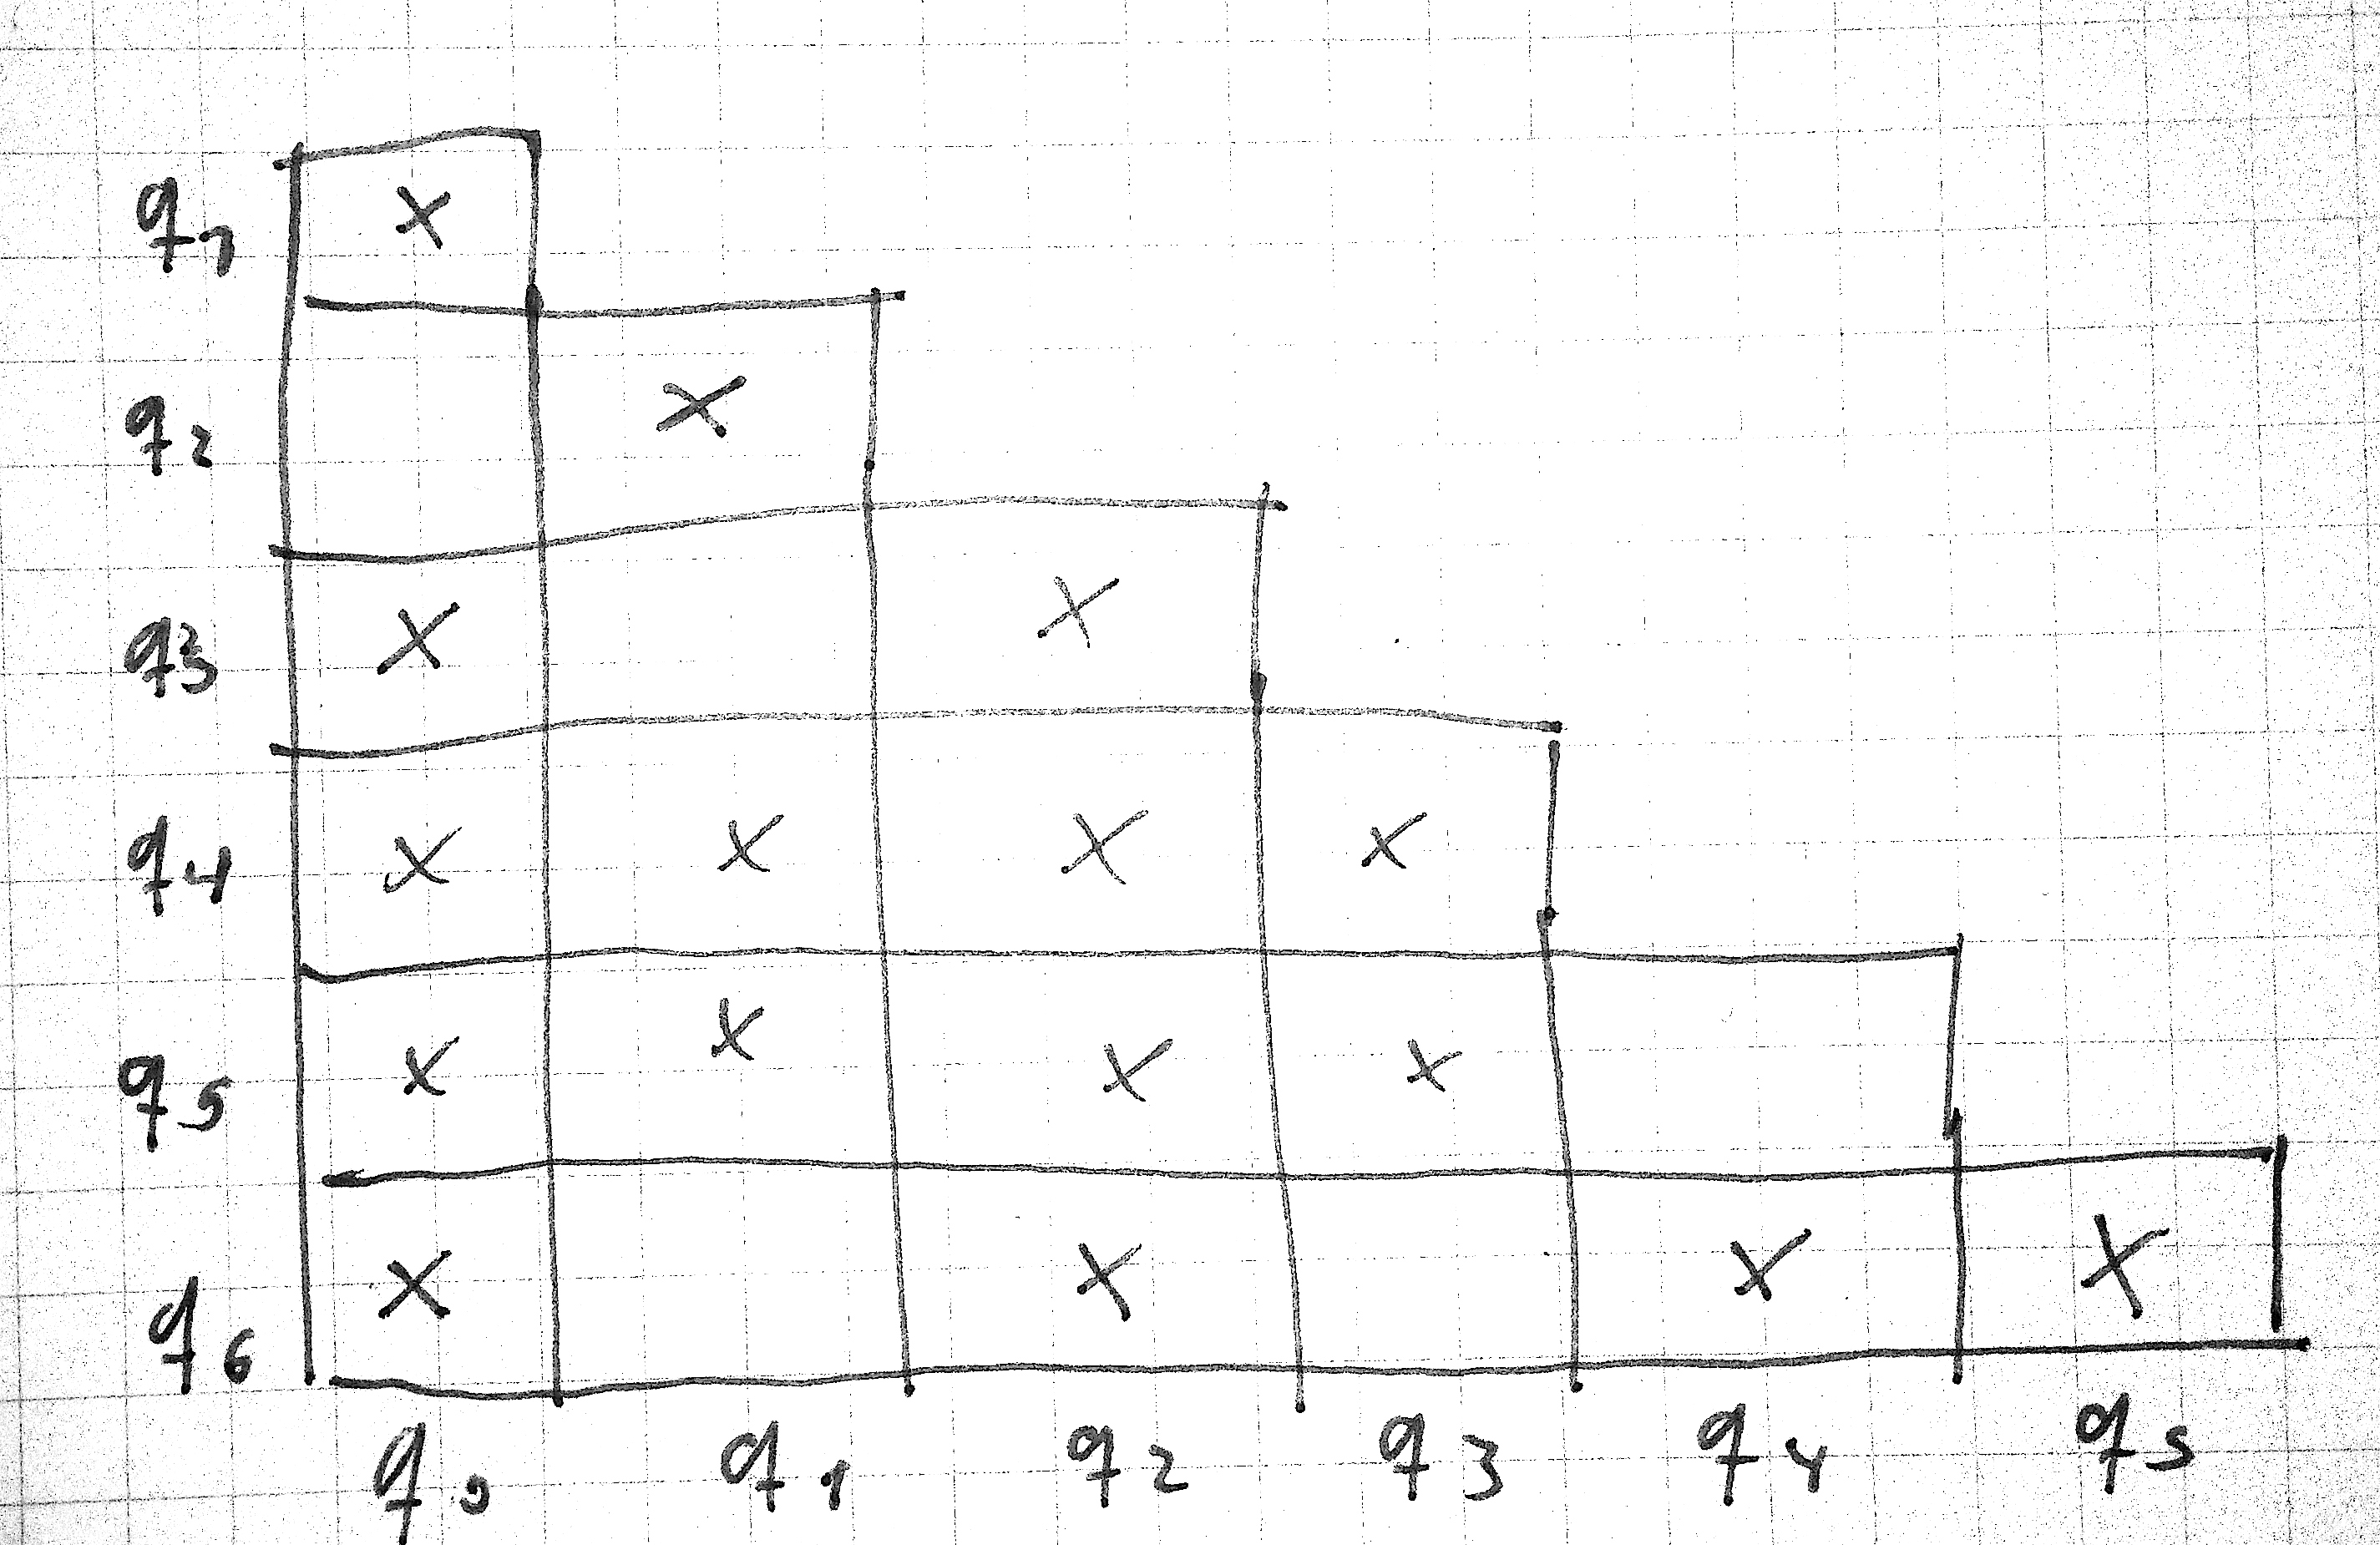
\includegraphics[width=0.8\linewidth]{table-filling}
    \caption{The result of the table filling algorithm. Squares marked with $x$ denote that the two states are distinguashable. In this completed table, all squares not marked indicate equivalent states.}
    \label{fig:table-filling}
\end{figure}

By theorem 4.20 in the course book, those states which have not found to be distinguishable are equivalent. By theorem 4.24, we can now go over all states $p$, find all the states equivalent to $p$ by looking for lack of a mark in the table, and group all those states equivalent to $p$ together with $p$ in a set, and let that set be a state in the minimized DFA. In this case, we get the following states:

\begin{align*}
    \begin{array}{c c c}
        \set{q_0,q_2} & \set{q_1,q_3,q_6} &\set{q_4,q_5}
    \end{array}
\end{align*}

We go over each of these new states in turn, and for each input symbol $a$ we determine the appropriate transition. We do this by picking any state in the old DFA in the set, for example the one with the lowest ordinal, call it $i$. We then create an arc labeled $a$ from the set containing $q_i$ to the one containing $\delta(q_i,a)$. We let the start state of our minimized DFA be the one containg the start state of the old DFA. The equivalence of states within the sets guarantee that we only need to look at the transitions from one state in the set, and the resulting transition will be valid for all the others as well.

We end up with the automaton

\begin{align*}
\centering
    \begin{array}{r || c | c}
        & a & b \\ \hline
        \to \set{q_0, q_2} & \set{q_1,q_3,q_6} & \set{q_4, q_5} \\
        \set{q_1,q_3,q_6}  & \set{q_1,q_3,q_6} &\set{q_1,q_3,q_6} \\
        ^*\set{q_4, q_5} & \set{q_0, q_2} & \set{q_4, q_5}
    \end{array}
\end{align*}

This is the minimized version of the original DFA, and thus the smallest possible DFA for that language.

\end{document}
